
%(BEGIN_QUESTION)
% Copyright 2010, Tony R. Kuphaldt, released under the Creative Commons Attribution License (v 1.0)
% This means you may do almost anything with this work of mine, so long as you give me proper credit

Anta at meteret i denne Wheatstone-brokretsen står i fullt utslag selv når RTD-en er ved 0$^{o}$ C (når broen burde være i balanse), med polaritet over voltmeterterminalene som vist.  Med ditt digitale multimeter måler du 100 millivolt mellom testpunktene {\bf B} og {\bf D}:

$$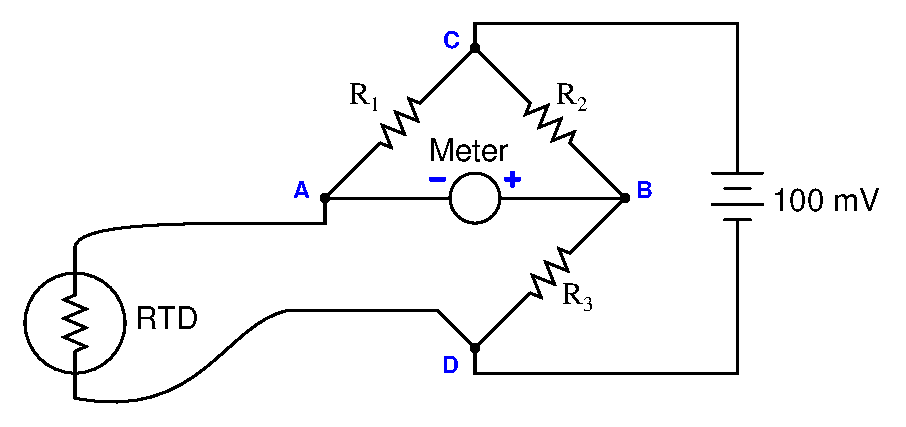
\includegraphics[width=15.5cm]{i00176x01.eps}$$

Vurder sannsynligheten for hver oppgitt feil i denne kretsen.  Vurder en og en feil (ingen samtidige feil), og avgjør om hver feil alene kan forklare \textit{alle} målinger og symptomer i kretsen.  

% No blank lines allowed between lines of an \halign structure!
% I use comments (%) instead, so that TeX doesn't choke.

$$\vbox{\offinterlineskip
\halign{\strut
\vrule \quad\hfil # \ \hfil & 
\vrule \quad\hfil # \ \hfil & 
\vrule \quad\hfil # \ \hfil \vrule \cr
\noalign{\hrule}
%
% First row
{\bf Fault} & {\bf Possible} & {\bf Impossible} \cr
%
\noalign{\hrule}
%
% Another row
$R_1$ failed open &  &  \cr
%
\noalign{\hrule}
%
% Another row
$R_2$ failed open &  &  \cr
%
\noalign{\hrule}
%
% Another row
$R_3$ failed open &  &  \cr
%
\noalign{\hrule}
%
% Another row
RTD failed open &  &  \cr
%
\noalign{\hrule}
%
% Another row
$R_1$ failed shorted &  &  \cr
%
\noalign{\hrule}
%
% Another row
$R_2$ failed shorted &  &  \cr
%
\noalign{\hrule}
%
% Another row
$R_3$ failed shorted &  &  \cr
%
\noalign{\hrule}
%
% Another row
RTD failed shorted &  &  \cr
%
\noalign{\hrule}
} % End of \halign 
}$$ % End of \vbox

\underbar{file i00176}
%(END_QUESTION)





%(BEGIN_ANSWER)

% No blank lines allowed between lines of an \halign structure!
% I use comments (%) instead, so that TeX doesn't choke.

$$\vbox{\offinterlineskip
\halign{\strut
\vrule \quad\hfil # \ \hfil & 
\vrule \quad\hfil # \ \hfil & 
\vrule \quad\hfil # \ \hfil \vrule \cr
\noalign{\hrule}
%
% First row
{\bf Fault} & {\bf Possible} & {\bf Impossible} \cr
%
\noalign{\hrule}
%
% Another row
$R_1$ failed open &  & $\surd$ \cr
%
\noalign{\hrule}
%
% Another row
$R_2$ failed open &  & $\surd$ \cr
%
\noalign{\hrule}
%
% Another row
$R_3$ failed open & $\surd$ &  \cr
%
\noalign{\hrule}
%
% Another row
RTD failed open &  & $\surd$ \cr
%
\noalign{\hrule}
%
% Another row
$R_1$ failed shorted &  & $\surd$ \cr
%
\noalign{\hrule}
%
% Another row
$R_2$ failed shorted & $\surd$ &  \cr
%
\noalign{\hrule}
%
% Another row
$R_3$ failed shorted &  & $\surd$ \cr
%
\noalign{\hrule}
%
% Another row
RTD failed shorted &  & $\surd$ \cr
%
\noalign{\hrule}
} % End of \halign 
}$$ % End of \vbox


%(END_ANSWER)





%(BEGIN_NOTES)

{\bf This question is intended for exams only and not worksheets!}.

%(END_NOTES)
